\documentclass[aspectratio=169,11pt]{beamer}
\usepackage{lmodern}
\usetheme[progressbar=frametitle,numbering=fraction]{metropolis}
\usepackage{amsmath,amssymb,bm}
\usepackage{listings,xcolor}
\usepackage{booktabs}
\definecolor{given}{HTML}{1F6FB2}
\definecolor{hand}{HTML}{2E7D32}
\definecolor{algo}{HTML}{B26A00}
\definecolor{impl}{HTML}{6A1B9A}
\lstset{language=Python,basicstyle=\ttfamily\footnotesize,keywordstyle=\color{impl}\bfseries,
  commentstyle=\color{gray},showstringspaces=false,columns=fullflexible,keepspaces=true}
% stage labels: every solution slide says which stage it is
\newcommand{\stage}[2]{{\color{#1}\bfseries\small\textsc{#2}}\par\smallskip}
\newcommand{\Byhand}{\stage{hand}{Step 1 -- by hand}}
\newcommand{\Algo}{\stage{algo}{Step 2 -- algorithm}}
\newcommand{\Impl}{\stage{impl}{Step 3 -- implementation}}
\newcommand{\Given}{\stage{given}{Recap}}
\newcommand{\Refresh}{\stage{given}{Refresher}}

\title{Exercise 2 -- Problems 2.1 and 2.3}
\subtitle{Principles of Machine Learning (MA-INF 4111), WS 2026/27}
\date{Solution slides}
\begin{document}
\maketitle

\begin{frame}{Roadmap}
\begin{enumerate}
\item \textbf{Refresher}: fitting a model to data; pdf, cdf and how they relate; least squares
\item \textbf{Problem 2.1}: recap; 2.1.1 load and plot the data; mini exercise $f=\mathrm dF/\mathrm dt$; 2.1.2 \texttt{weibull\_pdf()}, \texttt{weibull\_cdf()}
\item \textbf{Problem 2.3}: recap; 2.3.1 fit $A\,f(t\mid\alpha,\beta)$ with \texttt{curve\_fit()}; 2.3.2 plot, and compare with 2.2
\item \textbf{Takeaways}
\end{enumerate}
\bigskip
Every solution follows the same three steps:\\[3pt]
\textcolor{hand}{\textbf{by hand}} \;$\to$\; \textcolor{algo}{\textbf{algorithm}} \;$\to$\; \textcolor{impl}{\textbf{implementation}}
\end{frame}

% =====================================================================
\section{Refresher: what you should remember}

\begin{frame}{The big picture: fitting a model to data}\small
\Refresh
The whole sheet fits \textbf{one model} to \textbf{one data set} in six different ways. Every fit has four steps:
\begin{enumerate}
\item \textbf{Data:} observations, here weekly search counts $c_t$ at weeks $t=1,\dots,n$
\item \textbf{Model:} a family of curves with a few \emph{parameters}, here $f(t\mid\alpha,\beta)$
\item \textbf{Fit:} choose the parameters so that the curve matches the data as well as possible\\
\quad Problems 2.2--2.6: maximum likelihood, least squares, \dots; 2.7--2.8: ODEs, neural networks
\item \textbf{Interpret:} what do the fitted $\alpha,\beta$ say about the data?
\end{enumerate}
\medskip
\textbf{Problem 2.1 prepares steps 1 and 2:} load the data, implement the model.\\
The model is a \textbf{pdf} (with its \textbf{cdf}). To interpret a fit, you need to know what these are.
\end{frame}

\begin{frame}{Refresher: probability density function (pdf)}
\Refresh
Let $T$ be a \textbf{continuous random variable} with values in $[0,\infty)$.
\begin{enumerate}
\item A \textbf{pdf} is a function $f$ with \quad $f(t)\ge0$ \quad and \quad $\displaystyle\int_0^\infty f(t)\,\mathrm dt=1$
\item \textbf{Probability is area} under $f$:
\[P(a\le T\le b)=\int_a^b f(t)\,\mathrm dt\]
\item $f(t)$ itself is \textbf{not} a probability: $P(T=t)=0$, and $f(t)$ may exceed $1$.\\
It is probability \emph{per unit of $t$}: for a short interval $\Delta t$,
\[P(t\le T\le t+\Delta t)\approx f(t)\,\Delta t\]
\end{enumerate}
\end{frame}

\begin{frame}{Refresher: cumulative distribution function (cdf)}
\Refresh
\begin{enumerate}
\item The \textbf{cdf} accumulates probability up to $t$:
\[F(t)=P(T\le t)=\int_0^t f(s)\,\mathrm ds\]
\item Properties: $F(0)=0$,\quad $F$ never decreases,\quad $F(t)\to1$ for $t\to\infty$
\item Interval probabilities need no integral any more:
\[P(a<T\le b)=F(b)-F(a)\]
\item Quantiles: the \textbf{median} $t_{1/2}$ solves $F(t_{1/2})=\tfrac12$
\end{enumerate}
\end{frame}

\begin{frame}{Refresher: how pdf and cdf belong together}\small
\Refresh
\centering
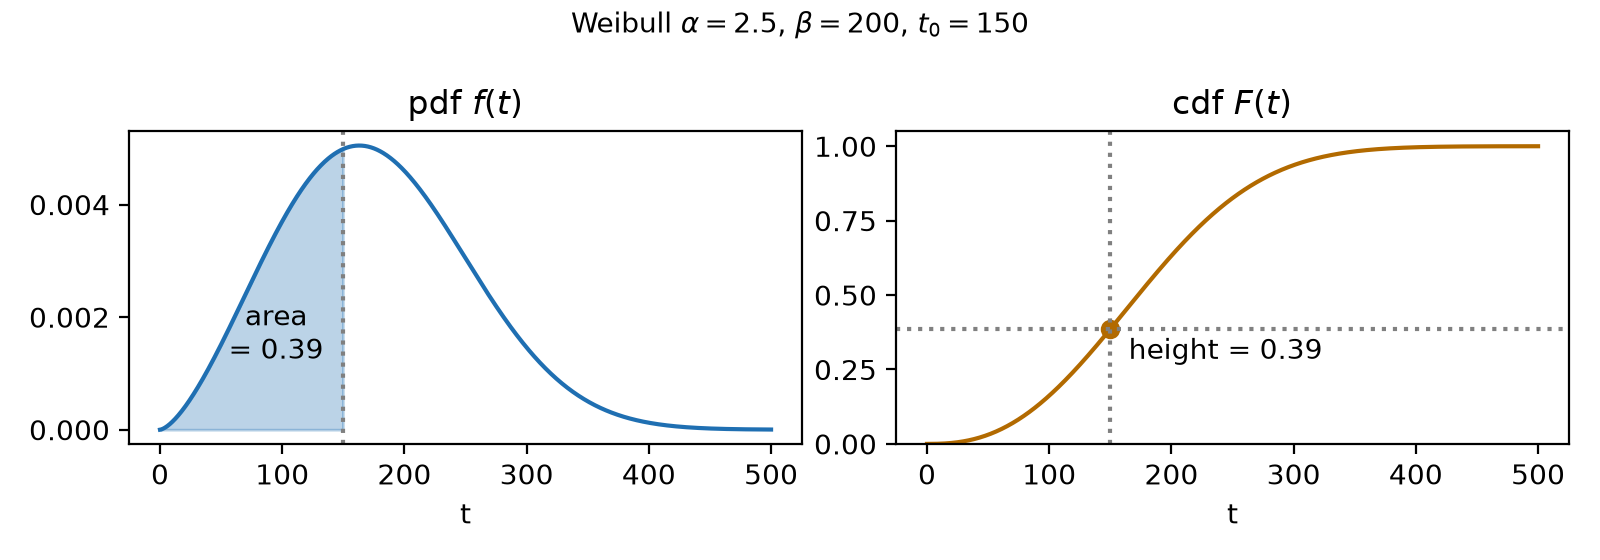
\includegraphics[width=.6\linewidth]{figures/refresher_pdf_cdf.png}
\[
F(t)=\int_0^t f(s)\,\mathrm ds
\quad\Longleftrightarrow\quad
f(t)=\frac{\mathrm dF}{\mathrm dt}(t)
\qquad\text{(fundamental theorem of calculus)}
\]
\raggedright
\begin{itemize}
\item Area under $f$ up to $t_0$ $=$ height of $F$ at $t_0$. $f\to F$: integrate; $F\to f$: differentiate
\item The mini exercise checks exactly this relation for the Weibull
\end{itemize}
\end{frame}

\begin{frame}{Refresher: least squares, step by step}
\Refresh
Data points $(t_i,y_i)$, $i=1,\dots,n$; a model curve $m(t\mid\bm\theta)$ with parameters $\bm\theta$.
\begin{enumerate}
\item \textbf{Residual} of point $i$: \quad $r_i(\bm\theta)=y_i-m(t_i\mid\bm\theta)$ \quad (vertical distance)
\item \textbf{Sum of squared residuals}:
\[S(\bm\theta)=\sum_{i=1}^n r_i(\bm\theta)^2\]
\item \textbf{Least squares}: choose $\hat{\bm\theta}=\arg\min_{\bm\theta} S(\bm\theta)$
\end{enumerate}
\medskip
Squares: positive and negative errors do not cancel, $S$ is differentiable, and large errors are punished most.\\
If $m$ is \textbf{linear} in $\bm\theta$: set $\nabla S=0$, closed form. If not: iterate.
\end{frame}

% =====================================================================
\section{Problem 2.1: recap of the task}

\begin{frame}{Given: the myspace data}
\Given
\begin{columns}[T]
\column{.42\textwidth}
\begin{itemize}
\item File \texttt{dataMyspace201303.csv}, Google Trends, retrieved March 2013
\item One row per \textbf{week}: \\ \texttt{2004-07-11 - 2004-07-17,1}
\item Column 1: date range (text) \\ Column 2: search count (number)
\item Counts are \textbf{relative}: Google rescales so that the maximum is $100$
\end{itemize}
\column{.56\textwidth}
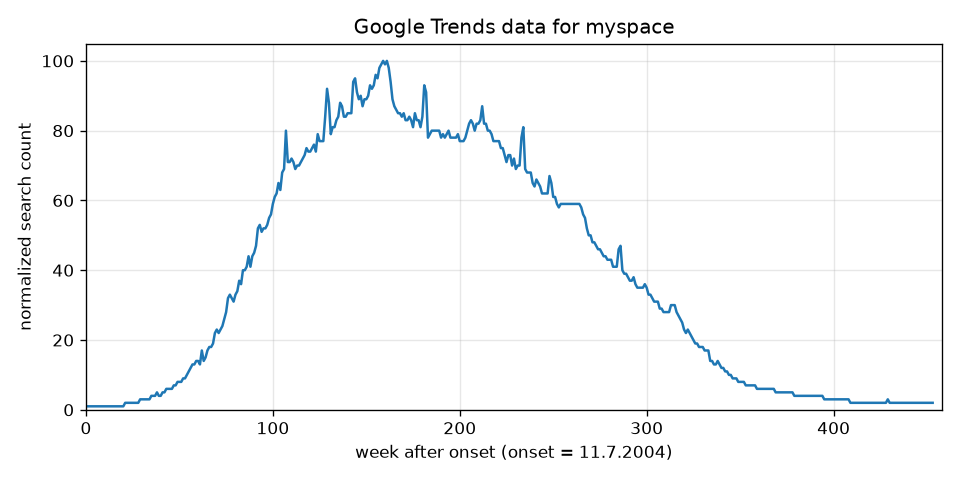
\includegraphics[width=\linewidth]{figures/task_2_1_1_data.png}
\end{columns}
\end{frame}

\begin{frame}{Background: why a Weibull?}
\Given
\begin{itemize}
\item The counts $c_t$ are a \textbf{histogram}: counts over discrete times $t$
\item Think of them as samples of an unknown (\emph{latent}) continuous density
\item The curve rises fast, peaks, then declines slowly $\Rightarrow$ \textbf{positively skewed}
\item A Gaussian is symmetric $\Rightarrow$ wrong model. We use the \textbf{Weibull}, $t\in[0,\infty)$:
\end{itemize}
\[
f(t\mid\alpha,\beta)=\frac{\alpha}{\beta}\Big(\frac t\beta\Big)^{\alpha-1}\exp\!\Big[-\Big(\frac t\beta\Big)^{\alpha}\Big]\quad(3)
\qquad
F(t\mid\alpha,\beta)=1-\exp\!\Big[-\Big(\frac t\beta\Big)^{\alpha}\Big]\quad(4)
\]
\begin{itemize}
\item $\alpha>0$: \textbf{shape},\quad $\beta>0$: \textbf{scale}
\end{itemize}
\end{frame}

\begin{frame}{Background: the Weibull describes rise and fall}
\Given
From (4): $\exp[-(t/\beta)^\alpha]=1-F(t)$. Insert this into (3):
\[
f(t)=\underbrace{\frac{\alpha}{\beta}\Big(\frac t\beta\Big)^{\alpha-1}}_{\text{growth term}}
\;-\;\underbrace{\frac{\alpha}{\beta}\Big(\frac t\beta\Big)^{\alpha-1}F(t)}_{\text{decline term}}\qquad(5)
\]
\begin{itemize}
\item Both terms are polynomial in $t$
\item $F(t)$ grows monotonically, so the decline term catches up over time
\item[$\Rightarrow$] the longer the process runs, the faster it declines: exactly the myspace story
\end{itemize}
\end{frame}

\begin{frame}{Problem to solve}\small
\Given
\begin{description}[Task 2.1.1]
\item[Task 2.1.1] Read column 2 into a numpy array, remove the \textbf{leading} zeros, call the rest
$\bm c=[c_1,\dots,c_n]$ and build $\bm t=[1,2,\dots,n]$ (start at $1$!). Plot $\bm c$ against $\bm t$.
Wrap both in reusable functions.
\item[Mini ex.] Using (3) and (4), show that $f=\dfrac{\mathrm dF}{\mathrm dt}$.
\item[Task 2.1.2] Implement (3) and (4) as numpy functions \texttt{weibull\_pdf()}, \texttt{weibull\_cdf()}
with explicit parameters $\alpha,\beta$. \textbf{Do not} use \texttt{scipy.stats}.
\end{description}
\end{frame}

% =====================================================================
\section{Task 2.1.1: load and plot the data}

\begin{frame}{2.1.1 -- by hand on a toy file}\small
\Byhand
Suppose column 2 of a tiny file reads
\[
\text{raw}=[\,0,\;0,\;0,\;1,\;3,\;0,\;2,\;5\,]
\]
\begin{enumerate}
\item First non-zero entry: position $4$ (value $1$). Three \textbf{leading} zeros.
\item Remove them: $\bm c=[1,\,3,\,0,\,2,\,5]$, so $n=5$.\\
\quad The zero \emph{inside} stays: it is a real measurement (a week with no searches).
\item Time steps: $\bm t=[1,2,3,4,5]$, \emph{not} $[0,\dots,4]$.
\item Plot the points $(t_i,c_i)$: $(1,1),(2,3),(3,0),(4,2),(5,5)$.
\end{enumerate}
\medskip
\alert{Why start at $t=1$?} Later we use $\log t$ and bins $(t_{j-1},t_j]$ with $t_0=0$; for $\alpha<1$ the density is infinite at $t=0$.
\end{frame}

\begin{frame}{2.1.1 -- the real file}
\Byhand
\begin{center}
\begin{tabular}{lr}
\toprule
rows in the file (weeks from 4.1.2004 to 16.3.2013) & $480$\\
leading zeros (4.1.2004 -- 10.7.2004) & $27$\\
remaining values $n$ & $480-27=453$\\
first week kept (onset) & 11.7.2004\\
$\max_t c_t$ & $100$ at $t=159$\\
zeros left inside $\bm c$ & none\\
\bottomrule
\end{tabular}
\end{center}
\medskip
Sanity checks: the onset matches the sheet (second week of July 2004), $n$ is ``slightly more than 400 weeks'', and the maximum is $100$ as Google's normalisation demands.
\end{frame}

\begin{frame}[fragile]{2.1.1 -- algorithm}
\Algo
\begin{enumerate}
\item Read column 2 of the csv as numbers: $\text{raw}_1,\dots,\text{raw}_N$
\item Find the first index with a positive value: $k=\min\{i:\text{raw}_i>0\}$
\item Keep everything from there on: $\bm c=[\text{raw}_k,\dots,\text{raw}_N]$, \;$n=N-k+1$
\item Build $\bm t=[1,\dots,n]$
\item Plot $\bm c$ over $\bm t$; label the axes ``week after onset'' and ``normalized search count''
\end{enumerate}
\medskip
\alert{Pitfall:} ``keep all $c_i>0$'' (a mask) would also delete interior zeros. We need ``cut off the front''.
\end{frame}

\begin{frame}[fragile]{2.1.1 -- implementation}
\Impl
\begin{columns}[T]
\column{.55\textwidth}
\begin{lstlisting}
def load_myspace_data(fname):
    raw = np.loadtxt(fname, delimiter=",",
                     usecols=1)   # column 2 only
    k = np.argmax(raw > 0)        # first True
    c = raw[k:]                   # cut the front
    t = np.arange(1, len(c) + 1)  # 1, ..., n
    return t, c

def plot_data(t, c):
    plt.plot(t, c)
    plt.xlabel("week after onset")
    plt.ylabel("normalized search count")
\end{lstlisting}
\column{.43\textwidth}
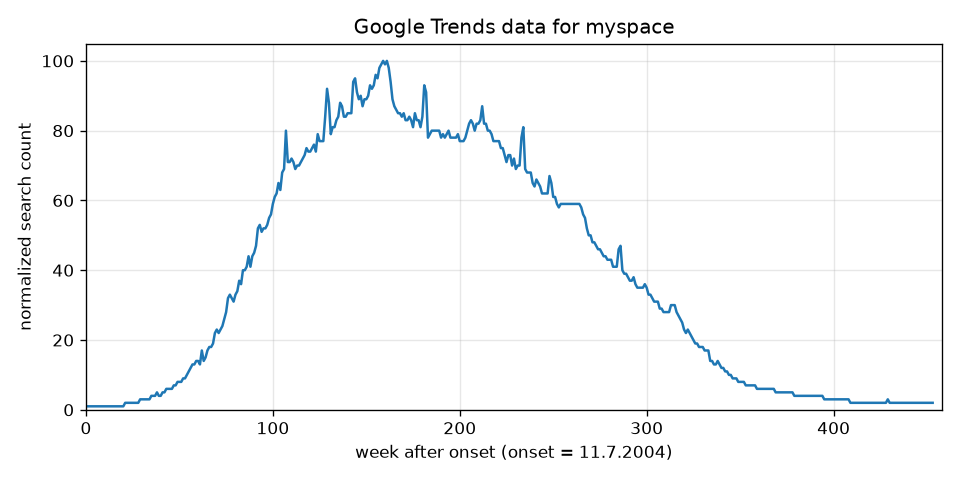
\includegraphics[width=\linewidth]{figures/task_2_1_1_data.png}
\small
\begin{itemize}
\item \texttt{usecols=1}: column 1 is text
\item \texttt{argmax} on booleans = first \texttt{True}
\end{itemize}
\end{columns}
\end{frame}

% =====================================================================
\section{Mini exercise: $f=\mathrm dF/\mathrm dt$}

\begin{frame}{Mini exercise -- by hand}
\Byhand
\textbf{Goal:} differentiate $F(t)=1-\exp[-(t/\beta)^\alpha]$ and get (3).
\begin{enumerate}
\item Name the inner function: $u(t)=\big(\tfrac t\beta\big)^{\alpha}$, so $F=1-e^{-u}$.
\item Derivative of $u$ (power rule, then inner factor $\tfrac1\beta$):
\[u'(t)=\alpha\Big(\frac t\beta\Big)^{\alpha-1}\cdot\frac1\beta\]
\item Chain rule: $\dfrac{\mathrm dF}{\mathrm dt}=0-e^{-u}\cdot(-u')=u'\,e^{-u}$
\item Insert:
\[\frac{\mathrm dF}{\mathrm dt}=\frac\alpha\beta\Big(\frac t\beta\Big)^{\alpha-1}\exp\!\Big[-\Big(\frac t\beta\Big)^{\alpha}\Big]=f(t\mid\alpha,\beta)\qquad\blacksquare\]
\end{enumerate}
\end{frame}

\begin{frame}{Mini exercise -- is $f$ a proper density?}
\Byhand
Because $f=F'$, the integral of $f$ is a difference of $F$-values:
\[
\int_0^\infty f(t)\,\mathrm dt=\lim_{t\to\infty}F(t)-F(0)
=\big(1-e^{-\infty}\big)-\big(1-e^{0}\big)=1-0=1
\]
(using $\alpha>0$, so $(t/\beta)^\alpha\to\infty$). Also $f\ge0$ everywhere.
\medskip
\begin{itemize}
\item[$\Rightarrow$] $f$ is a probability density, $F$ is its cumulative distribution
\item Typical mistake: forgetting the factor $\tfrac1\beta$ from the inner derivative
\end{itemize}
\end{frame}

\begin{frame}[fragile]{Mini exercise -- checking by computer}\small
\Algo
A derivation by hand can be checked in two independent ways:
\begin{enumerate}
\item \textbf{Symbolic:} let a computer algebra system compute $F'-f$ and simplify. Must give $0$.
\item \textbf{Numerical:} central difference $\dfrac{F(t+h)-F(t-h)}{2h}\approx f(t)$ for small $h$, at many $t$.
\end{enumerate}
\Impl
\begin{lstlisting}
t, a, b = sp.symbols("t alpha beta", positive=True)
F = 1 - sp.exp(-(t/b)**a)
f = a/b * (t/b)**(a-1) * sp.exp(-(t/b)**a)
sp.simplify(sp.diff(F, t) - f)        # -> 0
\end{lstlisting}
\small Numerically ($\alpha=2.5,\ \beta=200$, 50 points): largest error $9\cdot10^{-13}$; $\int_0^\infty f=1.0000$.
\end{frame}

% =====================================================================
\section{Task 2.1.2: \texttt{weibull\_pdf()} and \texttt{weibull\_cdf()}}

\begin{frame}{2.1.2 -- by hand: evaluate one point}
\Byhand
Take $\alpha=2,\ \beta=1,\ t=1$, so $t/\beta=1$:
\[
f(1\mid2,1)=\frac21\cdot1^{1}\cdot e^{-1^2}=2e^{-1}\approx0.736,
\qquad
F(1\mid2,1)=1-e^{-1}\approx0.632
\]
Special case $\alpha=1$: $f(t)=\tfrac1\beta e^{-t/\beta}$, the \textbf{exponential} distribution.
\medskip

These hand values become \textbf{test cases} for the code.
\end{frame}

\begin{frame}{2.1.2 -- by hand: what do $\alpha$ and $\beta$ do?}\small
\Byhand
\textbf{Scale $\beta$.} Write $s=t/\beta$. Then
\[f(t\mid\alpha,\beta)=\frac1\beta\,f\big(\tfrac t\beta\mid\alpha,1\big)\]
$\Rightarrow$ doubling $\beta$: curve twice as wide, half as high, area still $1$.

\textbf{Shape $\alpha$.} Where is the peak? Set $\frac{\mathrm d}{\mathrm dt}\log f=0$:
\[
\frac{\alpha-1}{t}-\frac{\alpha\,t^{\alpha-1}}{\beta^\alpha}=0
\;\Longrightarrow\;
t_{\text{mode}}=\beta\Big(\frac{\alpha-1}{\alpha}\Big)^{1/\alpha}\quad(\alpha>1)
\]
\begin{itemize}
\item $\alpha<1$: no peak, $f$ decreases and $f(0)=\infty$;\quad $\alpha=1$: exponential
\item $\alpha>1$: rises from $0$, one peak, then falls $\Rightarrow$ the myspace shape needs $\alpha>1$
\item Example $\alpha=2.5,\ \beta=2$: $t_{\text{mode}}=2\cdot0.6^{0.4}\approx1.63$
\end{itemize}
\end{frame}

\begin{frame}{2.1.2 -- algorithm}
\Algo
\begin{enumerate}
\item Inputs: times $t$ (a number or an array), shape $\alpha>0$, scale $\beta>0$
\item Compute $s=t/\beta$ elementwise
\item pdf: return $\frac\alpha\beta\,s^{\alpha-1}e^{-s^\alpha}$;\quad cdf: return $1-e^{-s^\alpha}$
\end{enumerate}
\medskip
Design choices:
\begin{itemize}
\item work elementwise on arrays (numpy broadcasting): one call evaluates the whole curve
\item $\alpha,\beta$ are explicit arguments, so later tasks can try many parameter values
\item $t=0$ with $\alpha<1$ gives $\infty$: mathematically correct, not a bug
\end{itemize}
\end{frame}

\begin{frame}[fragile]{2.1.2 -- implementation}
\Impl
\begin{lstlisting}
def weibull_pdf(t, alpha, beta):
    s = np.asarray(t, dtype=float) / beta     # works for numbers and arrays
    return alpha/beta * s**(alpha-1) * np.exp(-s**alpha)

def weibull_cdf(t, alpha, beta):
    s = np.asarray(t, dtype=float) / beta
    return 1.0 - np.exp(-s**alpha)

weibull_pdf(1, 2, 1)   # 0.7358  = 2/e      (our hand value)
weibull_cdf(1, 2, 1)   # 0.6321  = 1 - 1/e  (our hand value)
\end{lstlisting}
\small Extra check: agrees with \texttt{scipy.stats.weibull\_min(c=$\alpha$, scale=$\beta$)} up to $10^{-18}$ (used only as a test).
\end{frame}

\begin{frame}{2.1.2 -- the sheet's plots confirm the hand analysis}
\Impl
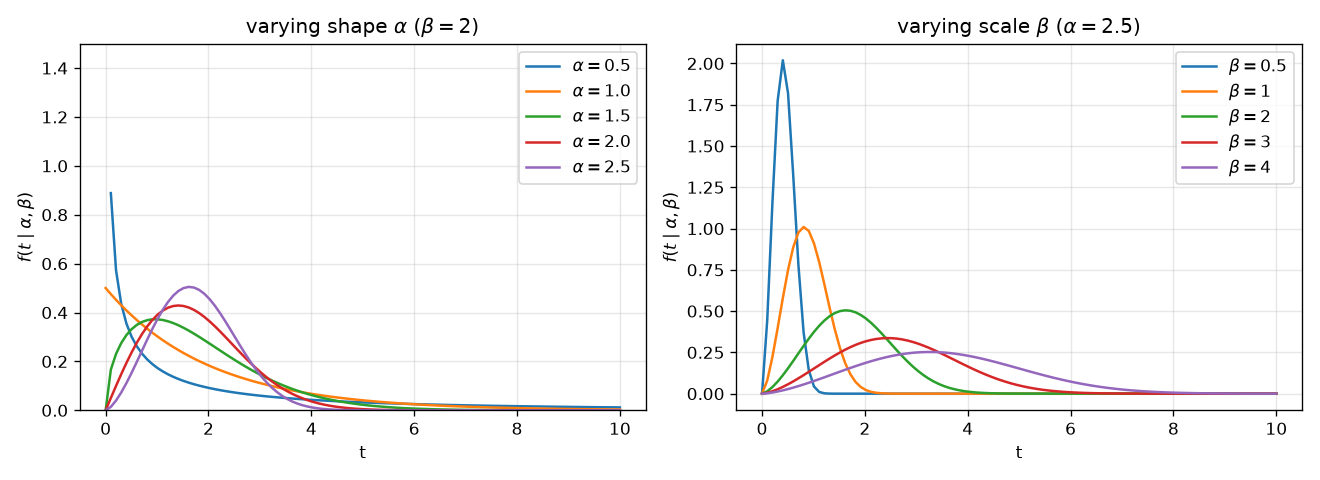
\includegraphics[width=\linewidth]{figures/task_2_1_2_shape_scale.png}
\small Left ($\beta=2$): $\alpha<1$ decreasing and infinite at $0$, $\alpha=1$ exponential, $\alpha>1$ one peak (for $\alpha=2.5$ at $1.63$).
Right ($\alpha=2.5$): larger $\beta$ = wider and lower, same area.
\end{frame}

% =====================================================================
\section{Problem 2.3: recap of the task}

\begin{frame}{Given}
\Given
\begin{itemize}
\item Data from 2.1: counts $\bm c=[c_1,\dots,c_n]$, weeks $\bm t=[1,\dots,n]$, $n=453$
\item Weibull pdf (3):\quad
$f(t\mid\alpha,\beta)=\dfrac{\alpha}{\beta}\Big(\dfrac t\beta\Big)^{\alpha-1}\exp\!\Big[-\Big(\dfrac t\beta\Big)^{\alpha}\Big]$,\quad $\alpha,\beta>0$
\item Our \texttt{weibull\_pdf(t, alpha, beta)} from 2.1.2
\item Result of 2.2 (Newton / MLE): $\hat\alpha=2.809$, $\hat\beta=215.43$
\item \texttt{scipy.optimize.curve\_fit(f, xdata, ydata, p0, bounds)}: least squares fit of a curve to points
\end{itemize}
\end{frame}

\begin{frame}{Problem to solve}\small
\Given
\begin{description}[Task 2.3.2]
\item[Task 2.3.1] Fit the \textbf{scaled Weibull}
\[\tilde f(t\mid A,\alpha,\beta)=A\cdot f(t\mid\alpha,\beta)\qquad(11)\]
to $(\bm t,\bm c)$ with \texttt{curve\_fit()}. Initial guesses (12): $\alpha=2$, $\beta=200$, $A=1000$.
Tell \texttt{curve\_fit()} that $\alpha,\beta$ must be \textbf{positive} (bounds). Report $\hat\alpha,\hat\beta$.
\item[Task 2.3.2] Plot the fitted model together with the data.
\end{description}
\medskip
The sheet warns: (a) this is a \emph{hack}, (b) the result will \emph{not} equal 2.2. We explain both.
\end{frame}

% =====================================================================
\section{Task 2.3.1: fit with \texttt{curve\_fit()}}

\begin{frame}{2.3.1 -- what exactly is minimised?}
\Byhand
\texttt{curve\_fit} treats the counts as \textbf{points on a curve}, $y_t=c_t$, and minimises
\[
S(A,\alpha,\beta)=\sum_{t=1}^{n}\Big(c_t-A\,f(t\mid\alpha,\beta)\Big)^2
\]
\begin{itemize}
\item Three unknowns: $A$ (height), $\alpha$ (shape), $\beta$ (scale)
\item $S$ is \textbf{linear in $A$} but \textbf{nonlinear in $\alpha,\beta$} $\Rightarrow$ no closed form, iterate
\item Each \emph{week} counts once. Nothing here uses that $f$ is a probability density\\
$\Rightarrow$ the ``hack'': statistically, MLE (2.2) is the principled choice
\end{itemize}
\end{frame}

\begin{frame}{2.3.1 -- by hand: the best amplitude for a fixed shape}\small
\Byhand
Fix $\alpha,\beta$ and write $g_t=f(t\mid\alpha,\beta)$. Then $S(A)=\sum_t(c_t-Ag_t)^2$ is a parabola in $A$:
\[
\frac{\mathrm dS}{\mathrm dA}=-2\sum_t g_t\,(c_t-Ag_t)=0
\quad\Longrightarrow\quad
A^*=\frac{\sum_t c_tg_t}{\sum_t g_t^2}
\]
\textbf{Toy:} $\bm g=[0.25,\,0.5,\,0.25]$ (sums to 1), $\bm c=[2,\,4,\,3]$ (sums to 9).
\begin{enumerate}
\item $\sum c_tg_t=0.5+2+0.75=3.25$,\quad $\sum g_t^2=0.0625+0.25+0.0625=0.375$
\item $A^*=3.25/0.375=8.67$ \quad (close to $\sum c_t=9$, but not equal)
\item Residuals: $2-2.17=-0.17$,\; $4-4.33=-0.33$,\; $3-2.17=0.83$\quad$\Rightarrow S=0.83$
\end{enumerate}
\alert{Lesson:} $A$ is ``roughly the total count'', adjusted to fit the points best.
\end{frame}

\begin{frame}{2.3.1 -- by hand: the start (12) on the real data}
\Byhand
\begin{columns}[T]
\column{.42\textwidth}\small
\begin{itemize}
\item Start $A=1000,\alpha=2,\beta=200$:\\ curve peaks near $4$, data near $100$\\
$S=1\,042\,660$
\item Keep the shape, take the best $A$ (formula on the last slide):\\
$A^*=18\,331$, \quad $S=101\,626$
\item $A^*$ is close to $C=17\,293$: the amplitude is the easy part
\item What is left is the \textbf{shape}: $\alpha,\beta$
\end{itemize}
\column{.56\textwidth}
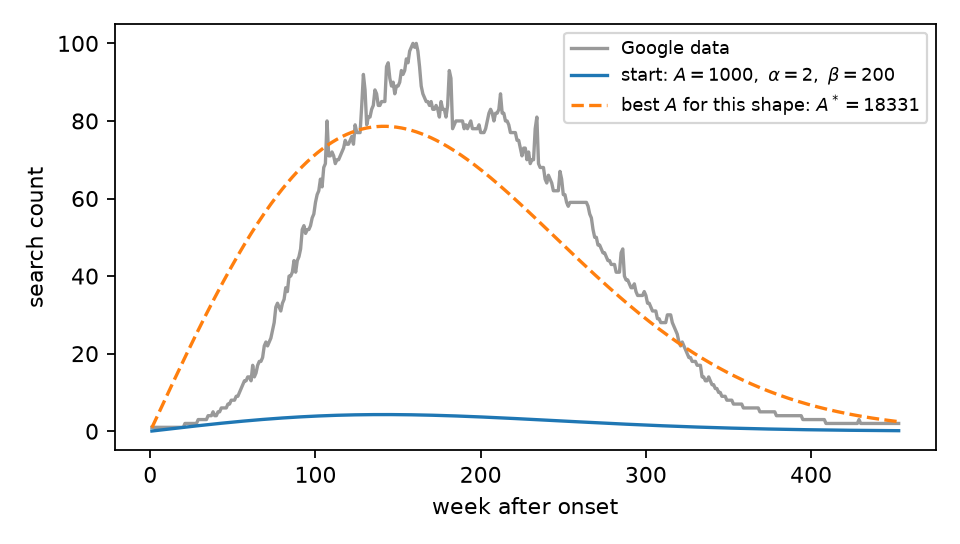
\includegraphics[width=\linewidth]{figures/start_guess.png}
\end{columns}
\end{frame}

\begin{frame}[fragile]{2.3.1 -- by hand: why the bounds are critical}
\Byhand
Try a step that overshoots to $\beta=-200$ with $\alpha=2.5$, at $t=100$:
\[
\Big(\frac{t}{\beta}\Big)^{\alpha-1}=(-0.5)^{1.5}=\;?\qquad\text{(no real number)}
\]
\begin{lstlisting}
>>> weibull_pdf(np.array([1., 100.]), 2.5, -200)
array([nan, nan])
\end{lstlisting}
\begin{itemize}
\item One \texttt{nan} in the residuals and the optimiser is lost
\item The optimiser does \textbf{not} know that $\alpha,\beta>0$: we must tell it
\item Lower bound $10^{-6}$, not $0$: $\beta=0$ divides by zero
\end{itemize}
\end{frame}

\begin{frame}{2.3.1 -- algorithm}\footnotesize
\Algo
\textbf{Input:} $\bm t,\bm c$, model $\tilde f$, start $\bm\theta_0=(A,\alpha,\beta)=(1000,2,200)$, bounds $\bm\theta>0$
\begin{enumerate}
\item Residual vector $\bm r(\bm\theta)=\bm c-\tilde f(\bm t\mid\bm\theta)\in\mathbb R^{n}$
\item Jacobian $J=\partial\bm r/\partial\bm\theta\in\mathbb R^{n\times3}$ (\texttt{curve\_fit}: finite differences)
\item Linearise $\bm r(\bm\theta+\bm\delta)\approx\bm r+J\bm\delta$ and solve the small least squares problem
\[\min_{\bm\delta}\ \|\bm r+J\bm\delta\|^2 \quad\text{(inside a trust region)}\]
\item Keep the step only if $S$ decreases and $\bm\theta+\bm\delta$ stays inside the bounds
\item Repeat until $S$ hardly changes (here: 23 evaluations)
\end{enumerate}
With bounds, \texttt{curve\_fit} uses the \emph{trust region reflective} method (\texttt{'trf'}),\\
without bounds Levenberg--Marquardt. Both are this Gauss--Newton idea plus safeguards.
\end{frame}

\begin{frame}[fragile]{2.3.1 -- implementation}
\Impl
\begin{lstlisting}
from scipy.optimize import curve_fit

def scaled_weibull(t, A, alpha, beta):      # model (11)
    return A * weibull_pdf(t, alpha, beta)

t, c = load_myspace_data()
p0     = [1000.0, 2.0, 200.0]                         # (12): A, alpha, beta
bounds = ([0.0, 1e-6, 1e-6], [np.inf, np.inf, np.inf]) # lower, upper
popt, pcov = curve_fit(scaled_weibull, t, c, p0=p0, bounds=bounds)
A, alpha, beta = popt
\end{lstlisting}
\footnotesize
\begin{itemize}
\item Order of \texttt{p0} and \texttt{bounds} $=$ order of the arguments \emph{after} \texttt{t}: \texttt{(A, alpha, beta)}
\item \texttt{bounds} is a pair \texttt{(lower, upper)}, one entry per parameter
\end{itemize}
\end{frame}

\begin{frame}{2.3.1 -- result and checks}
\Impl
\[
\boxed{\hat\alpha\approx2.731,\qquad\hat\beta\approx211.02,\qquad\hat A\approx17\,459}
\qquad S=13\,153
\]
\textbf{Checks}
\begin{itemize}
\item Other starts $(5000,1.5,100)$ and $(20000,3,250)$: same optimum to 6 digits
\item $\hat A/C=17459/17293=1.0096$: the amplitude is the total count, as expected
\item The MLE fit of 2.2 (scaled by $C$) has $S=15\,543>13\,153$: least squares wins \emph{its own} criterion
\item A bad start $(1,1,1)$ fails (``maximum number of function evaluations exceeded''):\\
$S$ is not convex, which is why the sheet hands us (12)
\end{itemize}
\end{frame}

% =====================================================================
\section{Task 2.3.2: plot, and compare with 2.2}

\begin{frame}[fragile]{2.3.2 -- plot the fitted model}
\Impl
\begin{columns}[T]
\column{.42\textwidth}
\begin{lstlisting}
plt.plot(t, c, label="Google data")
plt.plot(t, scaled_weibull(t, *popt),
         label="Weibull fit")
plt.legend()
\end{lstlisting}
\small
\begin{itemize}
\item No extra scaling: $\hat A$ is part of the model
\item Looks like the instructor's figure (sheet p.~10)
\end{itemize}
\column{.56\textwidth}
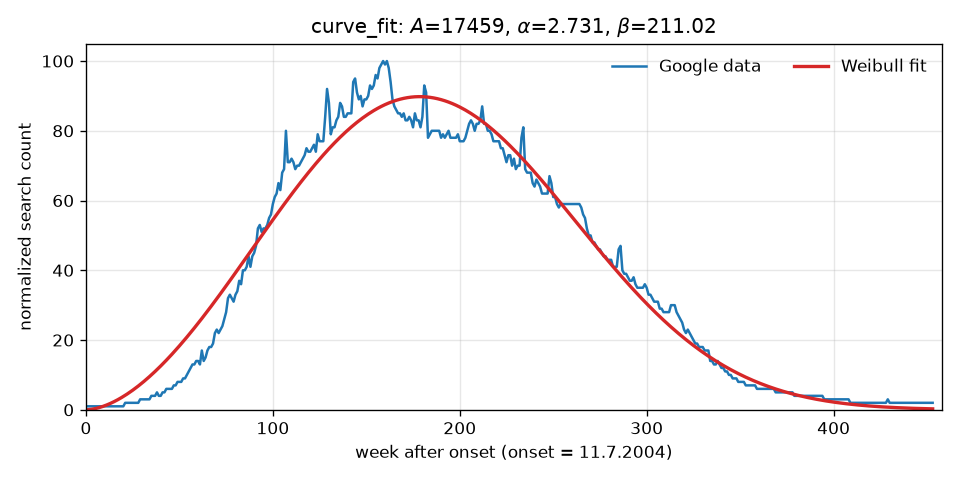
\includegraphics[width=\linewidth]{figures/task_2_3_2_curve_fit.png}
\end{columns}
\end{frame}

\begin{frame}{Why is the result not the same as in 2.2?}
\begin{center}
\begin{tabular}{lcc}
\toprule
& 2.2 Newton / MLE & 2.3 least squares\\
\midrule
objective & maximise $\sum_t c_t\log f(t)$ & minimise $\sum_t\big(c_t-Af(t)\big)^2$\\
each \dots\ counts once & search & week\\
errors measured & relative ($\log$) & absolute\\
height & fixed to $C$ & free parameter $A$\\
\midrule
$\hat\alpha$,\; $\hat\beta$ & $2.809$,\; $215.4$ & $2.731$,\; $211.0$\\
mode / peak height & week $184$ / $89.2$ & week $179$ / $89.8$\\
\bottomrule
\end{tabular}
\end{center}
\medskip
Different objectives $\Rightarrow$ different optima. Neither is a bug.
\end{frame}

\begin{frame}{Where does the difference come from?}
\begin{columns}[T]
\column{.40\textwidth}\small
\begin{itemize}
\item Squared errors are largest where counts are large: $92\%$ of $S$ comes from weeks $t\le250$
\item The long tail barely matters to least squares
\item So the curve moves towards the peak: \textbf{earlier and higher}
\item Residuals (bottom) are far from constant noise: the curve-fit ``hack'' ignores this
\end{itemize}
\column{.58\textwidth}
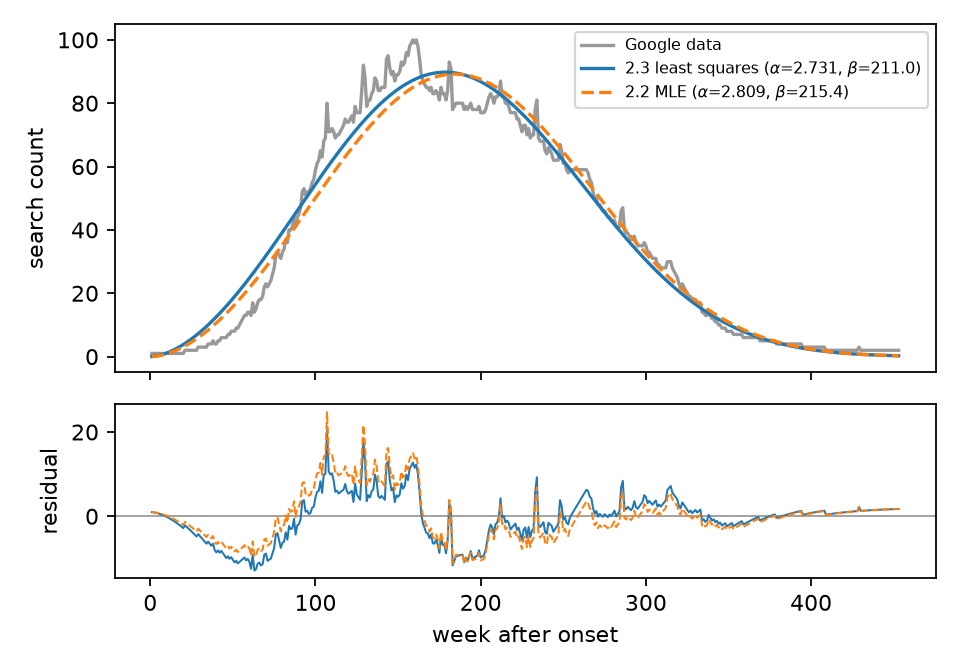
\includegraphics[width=\linewidth]{figures/ls_vs_mle.png}
\end{columns}
\end{frame}

% =====================================================================
\section{Takeaways}

\begin{frame}{Takeaways}\small
\begin{itemize}
\item Choose a model for the data's \textbf{shape} (skewed rise and fall): the Weibull is growth minus decline (5); $\alpha$ sets the form, $\beta$ only stretches time
\item Details matter: $\bm t$ starts at $1$; remove only \emph{leading} zeros; counts are relative (max $=100$)
\item A pdf has area $1$: to compare it with counts it needs an amplitude, $\hat A\approx\sum_tc_t$
\item Same model, different \textbf{criterion} (least squares vs.\ 2.2) $\Rightarrow$ different ``best'' parameters; least squares on a histogram is a quick hack
\item Nonlinear fits need \textbf{bounds} ($\alpha,\beta>0$) and a sensible \textbf{start}; check by restarting elsewhere
\item Check by hand, then by computer: symbolic, numerical, and against known values
\end{itemize}
\end{frame}

\end{document}
